% !TeX program = pdflatex
\documentclass[11pt]{amsart}

% Packages
\usepackage[dvipsnames]{xcolor}
\usepackage{enumitem}
\usepackage{amssymb,graphicx,mathtools}
\usepackage{float}
\usepackage{tikz}
\usetikzlibrary{calc,arrows.meta,decorations.markings}
\usepackage[margin=1in]{geometry}
\geometry{letterpaper}
\usepackage{etoolbox}

% Citations
\usepackage[square,longnamesfirst]{natbib}

% Theorem environments, numbered within sections on a shared counter
\theoremstyle{plain}
\newtheorem{theorem}{Theorem}[section]
\newtheorem{proposition}[theorem]{Proposition}
\newtheorem{corollary}[theorem]{Corollary}
\newtheorem{lemma}[theorem]{Lemma}
\theoremstyle{definition}
\newtheorem{remark}[theorem]{Remark}
\newtheorem{problem}{Problem}

% Load hyperref last
\usepackage[
citecolor=PineGreen,
colorlinks=true,
linkcolor=RoyalBlue,
urlcolor=BrickRed
]{hyperref}

\graphicspath{{figures/}}
\allowdisplaybreaks

% Commands
\newcommand{\Z}{\mathbb Z}
\newcommand{\R}{\mathbb R}
\newcommand{\T}{\mathbb T}
\newcommand{\E}{\mathbb E}
\renewcommand{\P}{\mathbb P}
\newcommand{\1}{\mathbf 1}
\newcommand{\ip}[2]{\langle #1,#2\rangle}
\newcommand{\norm}[1]{\lVert #1\rVert}
\newcommand{\abs}[1]{\lvert #1\rvert}
\newcommand{\dd}{\,\mathrm d}
\newcommand{\Hs}{\mathcal H}
\newcommand{\sgn}{\operatorname{sgn}}
\newcommand{\Hminus}[1]{\norm{#1}_{-1,\lambda}}
\newcommand{\Hplus}[1]{\norm{#1}_{1,\lambda}}
\newcommand{\defn}[1]{\textbf{#1}}

% Figure styles
\tikzset{
  ledge/.style={draw=black!22,line width=0.5pt},
  lvert/.style={circle,fill=black,inner sep=1.1pt}
}

\setcounter{secnumdepth}{3}

% No upper case on the title page
\makeatletter
\patchcmd{\@settitle}{\uppercasenonmath\@title}{\Large}{}{}
\patchcmd{\@setauthors}{\MakeUppercase}{\large}{}{}
\makeatother

\title{The randomly oriented Manhattan lattice in 2D is transient}
\author{Ahmed Bou-Rabee}
\author{Yuval Peres}

\begin{document}

\begin{abstract}
Independently orient each horizontal and vertical line of $\Z^2$ by a fair
coin.  A walker chooses one of the two lines through its current position
with equal probability and takes one step in the direction of that line.
Redner \citeyearpar{Red89} introduced this walk as a model of transport in
an isotropic random velocity field and predicted that its root-mean-square
displacement grows like $n^{2/3}$.  We prove that the walk is transient almost
surely.  The proof is a short variational argument.
\end{abstract}

\maketitle

\begin{figure}[!b]
\centering
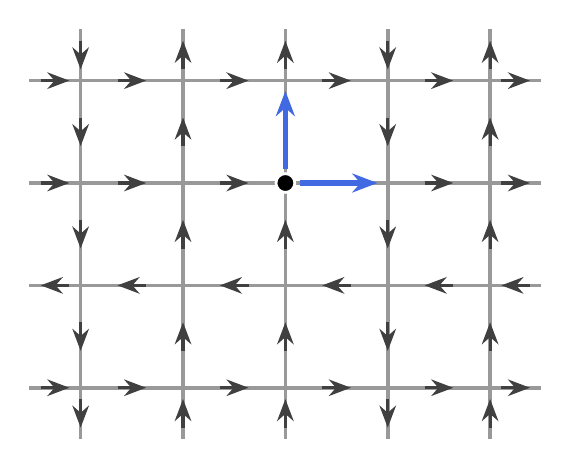
\begin{tikzpicture}[x=1.3cm,y=1.3cm,
  street/.style={draw=black!40,line width=1.3pt},
  head/.style={draw=black!75,line width=1.1pt,-{Stealth[length=2.8mm]}},
  move/.style={draw=RoyalBlue,line width=2.0pt,-{Stealth[length=3.2mm]}},
  site/.style={circle,fill=black,draw=white,line width=1.0pt,inner sep=2.4pt}]
\foreach \y in {0,...,3} \draw[street] (-0.5,\y) -- (4.5,\y);
\foreach \x in {0,...,4} \draw[street] (\x,-0.5) -- (\x,3.5);
% rows 0, 2, 3 run east and row 1 runs west; one head per edge
\foreach \y/\ms in {0/{-0.25,0.5,1.5,2.5,3.5,4.25},
                    2/{-0.25,0.5,1.5,3.5,4.25},
                    3/{-0.25,0.5,1.5,2.5,3.5,4.25}}
  \foreach \m in \ms \draw[head] (\m-0.14,\y) -- (\m+0.14,\y);
\foreach \m in {-0.25,0.5,1.5,2.5,3.5,4.25}
  \draw[head] (\m+0.14,1) -- (\m-0.14,1);
% columns 1, 2, 4 run north and columns 0, 3 run south
\foreach \x/\ms in {1/{-0.25,0.5,1.5,2.5,3.25},
                    2/{-0.25,0.5,1.5,3.25},
                    4/{-0.25,0.5,1.5,2.5,3.25}}
  \foreach \m in \ms \draw[head] (\x,\m-0.14) -- (\x,\m+0.14);
\foreach \x in {0,3} \foreach \m in {-0.25,0.5,1.5,2.5,3.25}
  \draw[head] (\x,\m+0.14) -- (\x,\m-0.14);
\draw[move] (2.14,2)--(2.90,2);
\draw[move] (2,2.14)--(2,2.90);
\node[site] at (2,2) {};
\end{tikzpicture}
\caption{One fair coin directs each line, so every edge of a line points the
same way.  The two blue arrows are the possible steps from the marked site.}
\label{fig:model}
\end{figure}

\section{Introduction}\label{sec:introduction}

The \defn{randomly oriented Manhattan lattice} is the square lattice with
every horizontal and vertical line given a direction by an independent fair
coin.  We study the random walk that at each step chooses one of the two
lines through its position with equal probability and moves one unit in that
line's direction (Figure~\ref{fig:model}).

One coin orients a whole line, so the environment has infinite-range
correlations: whenever the walk returns to a line it has visited before, it is
pushed in the same direction again.  Redner's heuristic in
Section~\ref{sssec:oriented} turns this repetition into the predicted
exponent, and the same feature places the two-dimensional model outside the
general theory recalled in Section~\ref{sssec:divfree}.
Figure~\ref{fig:path} compares the walk with simple random walk at two time
scales.  

\begin{figure}[t]
\centering
\includegraphics[width=0.95\textwidth]{fig_paths.pdf}
\caption{The randomly oriented Manhattan walk on the left and simple random
walk on the right, after $400$ steps in the top row and $4000$ steps in the
bottom row, colored by time from blue to red.  The two panels of each row are
drawn to the same scale.}
\label{fig:path}
\end{figure}

\citet*[p.~290]{Red89} introduced this walk as a model of transport in an
isotropic random velocity field, in work carried out with J.~Koplik,
F.~Leyvraz, and A.~Provata \citep*[p.~287]{Red89}, and predicted that its
root-mean-square displacement grows like $n^{2/3}$.
\citet*[p.~2506]{BGKPR90} presented this process as an example of a random walk
in a divergence-free random velocity field with long-range correlations.
\citet*[Section~1.4]{Tot18} lists this walk among the random walks with
stationary divergence-free drift, and \citet*[Section~3.5]{Pen20} lists the
model among open problems and conjectures the same displacement order
$n^{2/3}$.  \citet*[Appendix~A, Conjecture~1 and reference~\textup{[10]}]{Bos19}
records Guillotin-Plantard's transience conjecture and attributes it to her
2014 New Zealand Probability Workshop talk.
\citet*[p.~1]{CHT19} and \citet*[p.~1]{BH23} record transience as unresolved.

We prove this conjecture.  The proof bounds the annealed Green function by
evaluating a variational upper bound at an explicit function of
the orientations.

\subsection{Main results}\label{ssec:main-results}

Write $e_1$ and $e_2$ for the standard basis vectors of $\Z^2$.  Every line
of $\Z^2$ parallel to $e_1$ or to $e_2$ is given a direction by an
independent fair coin.  Record these choices in a function
$\omega\colon\Z^2\times\{1,2\}\to\{-1,1\}$, where $\omega(z,i)=1$ if the line
through $z$ parallel to $e_i$ points along $e_i$, and $\omega(z,i)=-1$
otherwise.  That line is unchanged when $z_i$ varies, so $\omega(z,i)$ does
not depend on $z_i$.  We call $\omega$ the \defn{environment} and write $\P$
for its law.

From $z$ the walker steps to
\begin{equation}\label{eq:rule}
  z+\omega(z,1)e_1\qquad\text{or}\qquad z+\omega(z,2)e_2,
  \qquad\text{with probability $1/2$ each.}
\end{equation}
Because $\omega(z,i)$ does not
depend on $z_i$, it agrees with $\omega(z-e_i,i)$, so the drift $\omega$ has
vanishing discrete divergence.  Every site therefore has two incoming and two
outgoing directed edges, and counting measure is invariant.

Write $P^\omega_z$ for the quenched law of the walk started at $z$ in a fixed
environment $\omega$, and write $p^\omega_n(z,z')$ for the probability under
$P^\omega_z$ that the walk is at $z'$ after $n$ steps.
Averaging over $\omega$ gives the annealed transition probability
$\overline p_n(z,z')=\E p^\omega_n(z,z')$.

\begin{theorem}\label{thm:main}
For $\P$-almost every environment $\omega$,
\[
  \sum_{n\geq0}p^\omega_n(x,x)<\infty\qquad\text{for every }x\in\Z^2\, .
\]
That is, the walk is transient in almost every environment.
\end{theorem}

We deduce Theorem~\ref{thm:main} from an annealed bound in continuous time.
Consider the continuous-time walk that jumps from $z$ to $z+\omega(z,i)e_i$
at rate $1$, for $i=1$ and $i=2$.  Its total jump rate is $2$, and its jump
chain is the walk in \eqref{eq:rule}.  Write
$p^\omega_t(z,z')$ for its transition probabilities and set
$\overline p_t(0,0)=\E p^\omega_t(0,0)$.

\begin{theorem}\label{thm:annealed}
There is a constant $C<\infty$ with
\[
  \int_0^\infty e^{-\lambda t}\overline p_t(0,0)\dd t\leq C
  \qquad\text{for all }\lambda\in(0,1]\, ,
\]
and hence $\int_0^\infty\overline p_t(0,0)\dd t<\infty$.
\end{theorem}

The continuous-time generator is the centered finite-difference
analogue of diffusion with drift: for every $h\colon\Z^2\to\R$,
\begin{equation}\label{eq:discrete-drift}
\begin{split}
  (\mathcal G_\omega h)(z)
  &=\frac12\sum_{i=1}^2
    \bigl[h(z+e_i)+h(z-e_i)-2h(z)\bigr]\\
  &\quad+\frac12\sum_{i=1}^2\omega(z,i)
    \bigl[h(z+e_i)-h(z-e_i)\bigr]\, .
\end{split}
\end{equation}
The first line is the symmetric simple-random-walk generator.  The second is
the centered first difference with coefficient $\omega$, and the vanishing
divergence noted above is its discrete incompressibility condition.

The randomness is essential.  Take instead the alternating orientations,
$\omega(z,1)=(-1)^{z_2}$ and $\omega(z,2)=(-1)^{z_1}$.  Then the
position at an even time, with each coordinate halved and rounded down,
performs simple random walk on $\Z^2$, so the walk is recurrent.  \citet*[p.~2]{BH23} report
this and attribute it to Guillotin-Plantard.

Equation~\eqref{eq:discrete-drift} also gives the comparison with a Brownian
particle in an incompressible random drift.  In the $d$-dimensional version,
the covariance of one component of $\omega$ is supported on its coordinate
axis.  Its average over a box of side $R$ has order $R^{1-d}$.  The average
over the same box of an isotropic covariance of order
$\abs{x-y}^{-2(1-\gamma)}$, as in \citet*[(1.2)]{ABK26}, has order
$R^{-2(1-\gamma)}$.  Matching these powers gives the heuristic
correspondence
\begin{equation}\label{eq:gamma-dimension}
  \gamma=\frac{3-d}{2}\, .
\end{equation}
Under this correspondence, the renormalization-group prediction
\citep*[(1.3)]{ABK26} gives variance of order $t^{4/3}$ in dimension two,
$t(\log t)^{1/2}$ in dimension three, and $t$ in dimensions at least four.
These are also the three regimes of the $\Hs_{-1}$ condition recorded in
\citet*[Section~1.4]{Tot18}.  We prove transience in dimension two by choosing
an explicit function in a variational upper bound for the Green
function.

\subsection{Related work}\label{ssec:related-work}

\subsubsection{Random walks on oriented lattices}\label{sssec:oriented}

Redner obtained the exponent $\nu=2/3$ by a heuristic self-consistency
argument \citep*[p.~290]{Red89}.  Suppose the horizontal displacement by
time $t$ has scale $R=R(t)$.  Among the $R$ vertical lines encountered,
the surplus pointing in one direction has order $\sqrt R$.  Treating each
line as visited about $t/R$ times gives a vertical displacement of order
$t/\sqrt R$.  Isotropy then gives $t/\sqrt R\approx R$, so
$R\approx t^{2/3}$.
 
In dimension $d$, the lines in one coordinate direction are indexed by
$d-1$ transverse coordinates.  The analogous volume count uses
$R(t)^{d-1}$ independent orientations and gives
\[
  R(t)\asymp tR(t)^{-(d-1)/2},
  \qquad\text{hence}\qquad
  \nu=\frac{2}{d+1}\, .
\]
Redner states this power-law prediction for $d\leq3$.
\citet*[p.~152, item~\textup{(v)} and (1.73a)--(1.73b)]{BG90} give the same
two-dimensional calculation and describe the model as following Redner.

In dimensions two and three, \citet*[Theorem~1.1 and the discussion following
it]{LTV18} proved two-sided bounds on the Laplace transform of the mean-square
displacement.  They also recorded the predicted orders
$t^{4/3}$ in dimension two and $t(\log t)^{1/2}$ in dimension three.  
\citet*[Theorem~1.1]{Ngu26} proved that, in dimension three, for every
$\varepsilon>0$ and all
sufficiently small $\lambda$,   this Laplace transform  is of order
$\lambda^{-2}\sqrt{\abs{\log\lambda}}$,
up to a multiplicative factor
$(\log\abs{\log\lambda})^{\pm(2+\varepsilon)}$.  This establishes the
leading logarithmic power predicted in
\citet*[discussion after Theorem~1.1]{LTV18}, with the stated correction
factors.


In the singly oriented analogue only the horizontal lines are directed, and
the vertical coordinate performs an autonomous random walk.  This model
has its continuum precursor in the layered flow of
\citet*[p.~901]{MdM80}; see also
\citet*[pp.~2--3]{LTV18}.  For the walk on $\Z^2$ that chooses uniformly
among its three outgoing edges, with independent fair horizontal
orientations and undirected vertical edges, \citet*[Theorem~1.8]{CP03}
proved almost-sure transience.
In a companion exposition, \citet*[Theorem~2.11]{CP04} also record that
this transient walk has zero speed.
\citet*[Section~2.1, Theorem~1 and (2.3)]{GLN08T} extended almost-sure
transience to horizontal orientations sampled independently conditional
on a measure-preserving dynamical system, and to their correlated
averages, under the integrability condition~(2.3).
For independent fair horizontal orientations,
\citet*[Theorem~2]{GLN08F} proved an annealed joint functional limit theorem
with horizontal scaling $n^{3/4}$ and vertical scaling $n^{1/2}$, and showed
that the two limiting components are dependent.
\citet*[Theorem~20 and Remark~21]{CGPS11} later proved a local limit
theorem and obtained return probability of order $n^{-5/4}$ along even
times; at odd times it is zero.
Fixing the orientations instead of sampling them leaves a Markov chain whose
transition law depends only on the height, and the walk above with any
prescribed sequence of orientations belongs to that stratified class
\citep*[p.~752]{Bre17}.  In every dimension, \citet*[Theorem~2.4 and
p.~753]{Bre17} gave a condition on such a chain that is necessary and
sufficient for recurrence, stated through the variance of a directional flux
that records how far the average horizontal flow of the levels spreads, and
presented that variance as a directional version of the macrodispersion
coefficients of the layered medium of \citet*[p.~901]{MdM80}.
\citet*[Example~1.4 and Theorem~1.7]{CP03} also proved transience for one
deterministic pattern, with the horizontal lines pointing east at nonnegative
heights and west below them.  For that lattice, \citet*[Theorem~1.2 and
Corollary~2.6]{BHP22} showed that the walk sits at the origin just after its
$2n$th vertical step with probability of order $n^{-3/2}$, and summed these
probabilities to recover transience, the criterion of
Theorem~\ref{thm:main}.  Orienting the vertical edges that leave the
horizontal axis, downward to the right of the origin and upward to the left,
makes the walk recurrent instead \citep*[Proposition~7.8]{Bre17}, and its
return time then exceeds $k$ with probability $(\log k)^{-1+o(1)}$
\citep*[Theorem~1.4]{BHP22}, so the edges at a single line already decide
recurrence.
These arguments use the autonomous vertical walk.  In the Manhattan model,
each coordinate is driven by the orientations encountered by the other;
our proof instead uses the expansion in independent line signs.
For the randomly oriented Manhattan lattice, simulations of
\citet*[Section~3.2]{MNOV20} indicate a return probability of order $n^{-4/3}$.

For  the classical Manhattan lattice with  alternating deterministic orientations, \citet*[Theorem~1]{BH23}
computed exactly the mean-square displacement.    That walk is
diffusive and recurrent, as recalled in Section~\ref{ssec:main-results}, so randomizing the orientations turns a recurrent walk into a transient one.  If a walker at $z$ instead moves deterministically to
$z+\omega(z,1)e_1+\omega(z,2)e_2$ at every step, then
\citet*[Theorem~1]{CHT19} proved that its trajectory is eventually
two-periodic.
\citet*[pp.~10251--10254]{BOC03}
study quantum and classical network models embedded in the deterministic
Manhattan lattice.

\subsubsection{Divergence-free drifts}\label{sssec:divfree}

Our walk belongs to the class of random walks in stationary doubly
stochastic environments; double stochasticity is the invariance of counting
measure noted above.
For walks whose transition probabilities admit a bounded cycle
representation, \citet*[Theorem~1.1 and assumptions~\textup{(a)--(c)},
p.~575]{DK08} proved a quenched invariance principle under ergodicity along
each coordinate direction, upper and lower bounds on the invariant density,
and uniform strong irreducibility.
Under the annealed law, the environment seen from the walker is stationary
and ergodic.  \citet*[Sections~1.1--1.2]{Tot18} treats these walks together
with diffusions in stationary incompressible random flows.

The $\Hs_{-1}$ condition asks that the drift covariance be integrable at low
frequencies.  It is equivalent to writing the drift as the divergence of a
stationary square-integrable antisymmetric matrix field, called its stream
matrix \citep*[Proposition~1\textup{(ii)}]{Tot18}.  Under
double stochasticity, zero annealed drift, ellipticity of the symmetric
rates, and the $\Hs_{-1}$ condition, \citet*[Theorem~1]{KT17} proved a central
limit theorem: the diffusively rescaled finite-dimensional distributions
converge to Brownian motion in probability with respect to the environment.  Under the additional
$L^{2+\varepsilon}$ integrability assumption on the stream matrix,
\citet*[Theorem~1\textup{(ii)}]{Tot18Q} proved the quenched central limit
theorem.  For the randomly oriented Manhattan lattice, the $\Hs_{-1}$
condition fails with a power-law divergence in dimension two, fails
logarithmically in dimension three, and holds in dimensions at least four
\citep*[Section~1.4]{Tot18}.  The theorems just quoted therefore do not apply
in dimensions two and three.
The relaxed sector condition of \citet*[Theorem~1]{HTV12} gives martingale
approximation and a central limit theorem for $\Hs_{-1}$ additive functionals
under strong convergence on a dense domain to an essentially
skew-self-adjoint operator; an extension
of this criterion underlies the proof in \citet*[Theorem~RSC2]{KT17}.
Our argument bounds the return resolvent directly by a finite-degree
candidate and does not require a martingale approximation or the
$\Hs_{-1}$ condition.

The continuum counterpart is a diffusion in an incompressible random drift.
Equation~\eqref{eq:discrete-drift} is the centered finite-difference version
of $\nu\Delta+f\cdot\nabla$ with $\nu=1/2$.  That operator generates
$\dd X_t=f(X_t)\dd t+\sqrt{2\nu}\dd W_t$
\citep*[(1.1)]{ABK26}.  An incompressible continuum drift is
written as $f=\nabla\cdot k$ for a stream matrix $k$, so its
generator is $\nabla\cdot(\nu I+k)\nabla$
\citep*[(1.9)]{ABK26}.  The same divergence-form operator appears in
\citet*[Theorem~1 and (1.2)--(1.5)]{Oel88}, who proved homogenization under
the square-integrability, regularity, and growth assumptions stated there.
For this continuum model, \citet*[Theorem~1\textup{(ii)}, pp.~1874--1877]{FK97}
proved a quenched invariance principle with a stationary stream matrix having
a finite $p$th moment for some $p>d$ and a square-integrable drift, under
the smoothness, growth, and ergodicity assumptions stated there.

For the Manhattan walk, define the discrete stream function by
\begin{equation}\label{eq:stream}
  \psi^\omega(z+e_2)-\psi^\omega(z)=\omega(z,1),
  \qquad
  \psi^\omega(z+e_1)-\psi^\omega(z)=-\omega(z,2),
  \qquad \psi^\omega(0)=0\, .
\end{equation}
Then $\omega$ is the rotated discrete gradient of $\psi^\omega$.  Along
each coordinate, $\psi^\omega$ is a sum of independent signs.  Formally
replacing these two random-walk partial sums by their Brownian scaling limits
gives
\[
  \psi(x,y)=W_1(y)-W_2(x),
  \qquad f=(\partial_y\psi,-\partial_x\psi)\, .
\]
Thus the two components of $f$ are constant along horizontal and vertical
lines, respectively, just as in the lattice model.

For the curl of the two-dimensional Gaussian free field,
\citet*[Theorem~1 and Remark~2]{TV12} proved superdiffusivity, with
Laplace-transform bounds corresponding to $t\log\log t$ and $t\log t$, and
predicted the order $t(\log t)^{1/2}$.
\citet*[Theorem~1.1]{CMOW25} proved that the mean-square displacement is of
that order.  \citet*[Theorem~A and Section~1.2]{ABK24} proved a quenched
invariance principle at this scaling, and identified the leading constant,
for their multiscale drifts with covariance decay $\abs{x-y}^{-2}$;
their equation~(1.3) predicts diffusive behavior for faster covariance decay
and superdiffusive behavior for slower decay.
\citet*[Theorem~A and assumptions~\textup{(J1)--(J4)}]{ABK26} proved
moment bounds for the quenched mean-square displacement at scale
$t^{2/(2-\gamma)}$, for their multiscale stream matrices with sufficiently
small Hurst exponent $\gamma>0$.
\citet*[Section~1.2]{ABK24} allows multiscale log-correlated, non-Gaussian
stream matrices and includes the mollified Gaussian free field.
\citet*[Section~1.5]{ABK26} instead assumes independent finite-range stream
increments at successive scales.  The stream function in
\eqref{eq:stream} has independent $\pm1$ increments along the two coordinate
axes.

\subsubsection{The variational formula}\label{sssec:variational}

When a diffusion in a divergence-free random flow rescales to a Brownian
motion, the covariance of that Brownian motion is called the effective
diffusivity.  Variational formulas for it are standard in homogenization.
\citet*[Section~V.1, (5.20)]{AM91} give a minimum principle for it, nonlocal
because a projection appears in the functional.
\citet*[Sections~4.1--4.2.1, (4.22) and (4.43)--(4.44)]{FP96} derive a min--max
principle for a stationary random flow, together with the minimum and maximum
principles that follow from it.  On the probability space of the flow,
\citet*[Proposition~5.1, (5.1)--(5.2)]{LOY98} give a
matching pair of supremum and infimum formulas.

We work with the resolvent at positive $\lambda$, without assuming a
diffusive limit.  For a generator $L=S+A$ with $S$ self-adjoint and $A$
skew-adjoint, \citet*[Theorem~4.1]{KLO12} express
$\operatorname{Re}\ip V{(\lambda I-L)^{-1}V}$ as an infimum of a quadratic
functional; the domain condition in that theorem is automatic here, because
the operators in this paper are bounded.  Closely related resolvent formulas
appear in \citet*[(2.17)]{LQSY04} and \citet*[(39)]{Tot18}, and
\citet*[Theorem~2.4 and Section~2.3]{GL14} prove a related min--max
principle for capacities of nonreversible Markov chains, with one boundary
set having finite complement.
For a one-dimensional self-repelling Brownian polymer in its stationary
Gaussian environment, \citet*[(92) and (98)--(100)]{TTV12} obtained
superdiffusive lower bounds by restricting a resolvent supremum to functions
of degree one.  In the Manhattan model,
\citet*[(1.7), (2.1), and Lemma~2.1]{LTV18} likewise evaluate the drift
resolvent at a degree-one test function to bound displacement from below.
Here the source is the constant at each spatial frequency, and we need an
upper bound on its resolvent.  The degree-three correction is determined
by the degree-one coefficient.  Parity makes the projection onto distinct
line indices preserve the required lowering exactly, whereas
\citet*[Sections~3--4]{LQSY04} control the exclusion of repeated indices
by comparison estimates.
For the two-dimensional asymmetric simple exclusion process at density
$1/2$ with generator~(1.5), \citet*[Theorems~1.1--1.2]{Yau04} proved
Laplace-transform bounds with logarithmic exponent $2/3$, up to subleading
factors.  The exponent $3/2$ in our resolvent denominator is another
logarithmic gain from estimates by degree, but concerns the return Green
function rather than the diffusion coefficient.

The same quadratic functional appears in quantitative homogenization, where
it is used to bound the effective diffusivity of a divergence-form operator.
\citet*[Exercise~10.1, immediately before (10.13)]{AKM19} record it for a
general coercive nonsymmetric bilinear form; taking that form to be
$\operatorname{Re}\ip v{(H+A_p)u}$, twice their functional at $(g,1)$ is the
right side of \eqref{eq:overview-bound}.  For symmetric coefficients
the corresponding pair is the Dirichlet energy and its convex dual, in
\citet*[(2.1)--(2.2)]{AS16} and \citet*[(2.6)--(2.9)]{AKM19}.  For
incompressible random drifts, \citet*[(2.4)--(2.5)]{ABK24} and
\citet*[(2.32)--(2.37)]{ABK26} take infima and suprema over a box to define a
diffusivity matrix at each scale.  Those works compare the variational quantities at
successive scales.  Here one real even function determines the candidate,
and integrating out its correction leaves the single weighted quadratic
problem in Lemma~\ref{lem:effective-energy}.

\subsection{Proof overview}\label{ssec:proof-overview}

Transience follows from the finiteness of the annealed Green function in
Theorem~\ref{thm:annealed}.  For a reversible walk such a bound is classically
obtained by exhibiting a unit flow of finite energy; see
e.g.\ \citet*[Theorem~2.11]{LP16}.  That criterion is usable because no
optimal flow is needed: any flow of finite energy gives the conclusion.  Our
walk is not reversible, so the criterion does not apply, but the argument
below has the same shape.  A variational upper bound reduces the proof to
exhibiting one function of the orientations.

The environment is invariant under translations of $\Z^2$, so a Fourier
transform in the position variable decomposes the Green function into an
integral over $p\in\T^2$ of resolvents $r_\lambda(p)$, one for each frequency,
and it suffices to bound these separately.  At a fixed $p$, split the
generator into a self-adjoint part $S_p$ and a skew-adjoint part $A_p$, and
put $H=\lambda I-S_p$.  Lemma~\ref{lem:variational-bound} gives, for every
$g\in L^2(\P)$,
\begin{equation}\label{eq:overview-bound}
  r_\lambda(p)\leq
  \ip g{Hg}+\ip{1-A_pg}{H^{-1}(1-A_pg)}\, .
\end{equation}
The first term measures the cost of $g$, the second the failure of $A_pg$
to equal the constant $1$.  We choose $g$ to make $A_pg$ nearly constant at
small cost.

Everything reduces to one scalar variational problem.  The candidate is built
from a single function $\varphi$ of one frequency, its degree-three part is
determined by $\varphi$, and the entire cost is an explicit quadratic in
$\varphi$ with a weight computed in closed form.  The rest of the proof sets
that quadratic up and minimizes it.

A function of the orientations depends on the infinitely many independent
signs carried by the lines, and expands in products of distinct signs, the
analogue of a Fourier series for coin flips.  Call the number of signs in a
product its degree.  Multiplying by one
orientation adds or removes a single sign, so $A_p$ carries each degree to
its two neighbours.  The constant $1$ in \eqref{eq:overview-bound} has degree
zero, so a competitor must have a degree-one part to meet it; that part then
leaves an error of degree two, which a degree-three part absorbs.  Its effect
is to add a positive multiplier to the degree-two weight, and the size of that
multiplier is where the logarithm comes from.  The three steps below carry
this out.

\medskip

\noindent\textbf{Step 1.}  Work in these coordinates.  Products of distinct
signs are orthogonal and $H$ preserves the degree, so both terms in
\eqref{eq:overview-bound} split into separate contributions from each degree.
Take $g$ with components of degrees one and three.

\medskip

\noindent\textbf{Step 2.}  Suppose $a=\abs{p_1}\geq\abs{p_2}$, and put
$\delta=\sqrt\lambda+a$.  For $\delta<1/256$, choose a real even
$\varphi\in L^2(\T,m)$ supported on
$\Gamma_\delta=\{\sqrt\delta\leq\abs r\leq1/4\}$.
The degree-one coefficient is $f=-i\varphi$, so its mixed residual is
$\sin(r)\varphi(r)$.  Minimizing a quadratic upper bound determines a
degree-three coefficient from this residual.  Oddness in the row frequency
and evenness of the weights give four exact cancellations in the proof of
Lemma~\ref{lem:parity}.

The resulting cost is bounded by the weight
\begin{equation}\label{eq:q}
  q(r)\coloneqq\frac{\abs r}{\sqrt{\log(1/\abs r)}}
  \qquad(0<\abs r\leq1/4)\, .
\end{equation}
This is the effective cost per squared row coefficient.
With $s=\sin p_1$ and $H_0=\lambda+\theta(p)$,
Lemma~\ref{lem:effective-energy} gives
\[
  r_\lambda(p)\leq
  \frac{\left(1-s\int_{\Gamma_\delta}\varphi\dd m\right)^2}{H_0}
  +C\int_{\Gamma_\delta}q(r)\varphi(r)^2\dd m(r)\, ,
\]
with $C=16$.
The first term charges the constant residual, and the second bounds
every other contribution to the candidate's cost.

\medskip

\noindent\textbf{Step 3.}  For a prescribed integral of $\varphi$,
Cauchy--Schwarz minimizes the weighted square integral at
$\varphi=t/q$ on $\Gamma_\delta$.
Writing $Z_\delta=\int_{\Gamma_\delta}q^{-1}\dd m$, the substitution
$u=\log(1/\abs r)$ turns $Z_\delta$ into an integral of $\sqrt u$.
Equation~\eqref{eq:Z} evaluates that integral exactly and gives
$Z_\delta\asymp[\log(1/\delta)]^{3/2}$.
Minimizing over $t\in\R$ gives
$r_\lambda(p)\leq(H_0+s^2Z_\delta/16)^{-1}$.
Together with the choice $g=0$ for the remaining frequencies, this proves
\eqref{eq:frequency-bound}.

The logarithmic exponent $3/2$ makes the frequency integral finite.
Taking $g=0$ alone gives $(\lambda+\theta(p))^{-1}$, whose integral
diverges logarithmically as $\lambda\downarrow0$.  In contrast, the bound
above gives the convergent integral
$\int_1^\infty u^{-3/2}\dd u$ after the substitution $u=1+\log(1/a)$.
The region $a\leq\sqrt\lambda$ has area $4\lambda$ and is bounded using
$r_\lambda(p)\leq1/\lambda$.  Thus the Green function is bounded uniformly
in $\lambda$.  Running the discrete walk with a rate-two Poisson clock gives
the continuous-time walk, whose Green function is half the discrete one,
so Theorem~\ref{thm:main} follows.
Sections~\ref{sec:variational}--\ref{sec:effective-energy} set the quadratic
up: Section~\ref{sec:variational} proves the variational bound,
Section~\ref{sec:coins} records the coordinates and operator formulas,
Section~\ref{sec:evaluation} builds the candidate from $\varphi$, and
Section~\ref{sec:effective-energy} computes its cost.
Section~\ref{sec:fixed-frequency} minimizes the quadratic and proves the two
main theorems.

\subsection{Formalization}\label{ssec:formalization}

Every theorem, lemma and proposition of this paper has been formalized in
Lean~4 and proved from Mathlib, together with the recurrence assertion in
Problem~\ref{prob:which}.  No proof uses an axiom beyond the three of Lean's
own logic, and no proof contains an incomplete step.  The development is at
\url{https://github.com/nitromannitol/Manhattan-Transience}.

The bytes of each formalized statement are pinned by a cryptographic hash
against the label of the result it transcribes, so a statement cannot be
weakened once it is proved, and a check confirms that every numbered result
here is covered.  Theorem~\ref{thm:main} is proved twice, once through the
competitor of Section~\ref{sec:evaluation} and once through a second competitor
that shares with it only Lemma~\ref{lem:variational-bound}.  P\'olya's theorem
in two dimensions is not available in Mathlib, so the recurrence in
Problem~\ref{prob:which} is proved there from the factorization of the walk
into two independent one-dimensional walks rather than quoted.

Every numbered statement is formalized as displayed.  The two constants
$C$ of Lemma~\ref{lem:effective-energy} and $C$ of
Proposition~\ref{prop:frequency} are universal but unspecified in those
statements, and the values $16$ and $2048$ recorded in the proofs are the ones
the arguments here produce.  The formalized proofs reach the same statements
along a lossier route and produce larger values, below $670$ in place of $16$
and correspondingly larger in place of $2048$: they split the residual by
Cauchy--Schwarz in the passage from Lemma~\ref{lem:parity} to
\eqref{eq:energy-reduction} and bound the degree-three form by a majorant
rather than minimizing it exactly.

\subsection{Notation and conventions}\label{ssec:notation}

\begin{itemize}
\item All torus integrals use the normalized Haar measure
$\dd m(s)=\dd s/2\pi$ on $\T=(-\pi,\pi]$, and $\dd m(p)=\dd m(p_1)\dd m(p_2)$
on $\T^2$.
\item $\ip\cdot\cdot$ and $\norm\cdot$ are the real or complex $L^2$ inner
product and norm on the space under discussion; complex inner products
are conjugate-linear in the first argument.
\item $c>0$ and $C>0$ denote finite constants whose value may change from
line to line.  Numerical constants used in the quantitative bounds are
displayed explicitly.
\end{itemize}

\section*{Acknowledgments}
The research of Y. Peres was supported by National Natural Science Foundation of China grant
RFIS-W2531011.  We acknowledge use of ChatGPT 5.6.

\section{The variational bound}\label{sec:variational}

We express the annealed Green function as an integral of resolvents and
bound each resolvent by the cost of a single function.

\subsection{Fourier transform}\label{ssec:fourier}

Translations of the environment describe the environment seen from the
walker.  For $x\in\Z^2$, set
\[
  (T_xF)(\omega)=F(\tau_x\omega),\qquad
  (\tau_x\omega)(z,i)=\omega(z+x,i)\, .
\]
The operator $T_x$ is unitary on $L^2(\P)$, and $T_{\pm e_i}$ commutes
with multiplication by $\omega(0,i)$ because that sign is constant along
the line parallel to $e_i$.

On $L^2(\P;\ell^2(\Z^2))$, the environment seen from the walker together
with its position has generator
\begin{equation}\label{eq:joint-generator}
  (\mathcal GF)(\omega,z)=\sum_{i=1}^2
  \bigl[F(\tau_{\omega(0,i)e_i}\omega,z+\omega(0,i)e_i)-F(\omega,z)\bigr]\, .
\end{equation}
Each jump shifts both the position and the environment viewed from it.
To extract returns to the origin, set
$\delta_0(\omega,z)=\1_{\{z=0\}}$.  Then
\begin{equation}\label{eq:return-correlation}
  \overline p_t(0,0)=\ip{\delta_0}{e^{t\mathcal G}\delta_0}\, .
\end{equation}
The inner product averages the probability of returning over the initial
environment.
Under the Fourier transform
$\widehat F(\omega,p)=\sum_z e^{-ip\cdot z}F(\omega,z)$, the function
$F(\tau_x\omega,z+x)$ becomes $e^{ip\cdot x}T_x\widehat F$.

\begin{proposition}\label{prop:generator}
For every $p\in\T^2$, the Fourier transform of $\mathcal G$ is
$G_p=S_p+A_p$, where
\begin{align}
  S_p&=\frac12\sum_{i=1}^2
  \bigl(e^{ip_i}T_{e_i}+e^{-ip_i}T_{-e_i}-2I\bigr),\label{eq:Sp}\\
  A_p&=\frac12\sum_{i=1}^2\omega(0,i)
  \bigl(e^{ip_i}T_{e_i}-e^{-ip_i}T_{-e_i}\bigr)\, .\label{eq:Ap}
\end{align}
The first operator averages the two directions on each axis; the second
weights their difference by the line sign.
Uniformly in $p$, the operator $S_p$ is self-adjoint and nonpositive,
$A_p^*=-A_p$, $\norm{S_p}\leq4$, and $\norm{A_p}\leq2$.
Put $d(s)=1-\cos s$ and $\theta(p)=d(p_1)+d(p_2)$.
For every $\lambda>0$,
\begin{align}
  \int_0^\infty e^{-\lambda t}\overline p_t(0,0)\dd t
  &=\int_{\T^2}r_\lambda(p)\dd m(p),\label{eq:green}\\
  r_\lambda(p)&\coloneqq
  \operatorname{Re}\ip1{(\lambda I-G_p)^{-1}1}\, .\label{eq:frequency-resolvent}
\end{align}
The Green function is therefore the average of one scalar resolvent for
each spatial frequency.
\end{proposition}

\begin{proof}
Splitting \eqref{eq:joint-generator} according to the two values of each
sign gives \eqref{eq:Sp} and \eqref{eq:Ap}.  Unitarity of the shifts and
their commutation with the corresponding signs give the operator
assertions.  The Fourier transform of $\delta_0$ is $1$, so Plancherel's
theorem and integration of \eqref{eq:return-correlation} against
$e^{-\lambda t}\dd t$ give \eqref{eq:green}.
\end{proof}

\subsection{The fixed-frequency bound}\label{ssec:varbound}

The positive symmetric part supplies the two norms used to measure the
competitor and its residual.  Fix $\lambda>0$ and $p\in\T^2$, and put
\begin{equation}\label{eq:H}
  H\coloneqq\lambda I-S_p,\qquad
  \lambda I\leq H\leq(\lambda+4)I,\qquad
  H1=(\lambda+\theta(p))1\, .
\end{equation}
Thus $H^{-1}$ and $H^{-1/2}$ are bounded, and we set
\begin{equation}\label{eq:Hnorms}
  \Hplus g^2\coloneqq\ip g{Hg},\qquad
  \Hminus u^2\coloneqq\ip u{H^{-1}u}\, .
\end{equation}
The first norm charges the candidate for its energy; the second measures
its residual with the reciprocal weight.

\begin{lemma}\label{lem:variational-bound}
For every $\lambda>0$, $p\in\T^2$, and $g\in L^2(\P)$,
\begin{equation}\label{eq:var}
  0\leq r_\lambda(p)\leq\Hplus g^2+\Hminus{1-A_pg}^2\, .
\end{equation}
The cost of any candidate bounds the resolvent, with coefficient
$1$ independently of $\lambda$, $p$, and $g$.
\end{lemma}

\begin{proof}
Compare the candidate with the exact resolvent vector
$z=(H-A_p)^{-1}1$, and abbreviate $d=z+g$ and $q=1-A_pg$.  Since
$1=Hz-A_pz$, subtracting $A_pg$ from both sides gives $q=Hz-A_pd$.
A skew-adjoint operator has $\operatorname{Re}\ip{A_pu}u=0$ for every $u$,
which removes the diagonal terms and leaves
\[
  r_\lambda(p)=\operatorname{Re}\ip1z=\Hplus z^2,
  \qquad
  \operatorname{Re}\ip qd=\operatorname{Re}\ip{Hz}d\, .
\]
Now write $z=d-g$ and expand, using that $H$ is self-adjoint:
\[
  \Hplus z^2=\Hplus g^2
  +\left(2\operatorname{Re}\ip qd-\Hplus d^2\right)\, .
\]
The bracket is at most $\Hminus q^2$, because
$2\operatorname{Re}\ip qd\leq\Hminus q^2+\Hplus d^2$ is the weighted
Cauchy--Schwarz inequality for the dual pair $\Hplus\cdot$, $\Hminus\cdot$.
This is the stated bound.  No normalization of $g$ is used.
\end{proof}

\begin{remark}
Taking $g=0$ gives
\begin{equation}\label{eq:zero-function}
  r_\lambda(p)\leq\Hplus0^2+\Hminus1^2
  =\frac1{\lambda+\theta(p)}\, .
\end{equation}
This bound will suffice away from the small frequencies.
\end{remark}

Without the variational upper bound, constructing a function with finite
cost would not control the Green function of this nonreversible walk.

\section{Fourier--Walsh coordinates}\label{sec:coins}

We separate the cost in \eqref{eq:var} by the number of line signs in
each product.  Fix $p\in\T^2$ and write $A=A_p$.

Products of distinct independent signs form an orthonormal basis for
functions of finitely many signs.  Conditional expectation onto increasing
finite sets of signs and $L^2$ martingale convergence extend this basis to
$L^2(\P)$; see \citet*[Theorem~1.5]{ODo14} for the finite-dimensional
Fourier--Walsh expansion.

\subsection{Degree and frequency}\label{ssec:degree}

Line indices distinguish the independent signs on which the candidate
depends.
Index each line sign by $(x,j)$, where $j\in\{1,2\}$ and
$x\in\{z\in\Z^2:z_j=0\}$.  A sign of type $1$ is a row sign,
and a sign of type $2$ is a column sign.  Let $\Hs_n$ be the closed span of
products of $n$ distinct line signs.  Every $F\in\Hs_n$ has a symmetric
coefficient $f$ such that
\[
  F(\omega)=\sum_{\mathbf x,\mathbf j}f_{\mathbf j}(\mathbf x)
  \prod_{a=1}^n\omega(x_a,j_a)\, .
\]
The sum runs over ordered line indices; $f$ vanishes when two coincide,
so each product contains exactly $n$ distinct signs.
If $F\in\Hs_n$ and
$G\in\Hs_m$ have coefficients $f$ and $g$, then
\begin{equation}\label{eq:iso}
  \ip FG=\1_{\{m=n\}}n!\ip fg_{\ell^2}\, .
\end{equation}
Different degrees are orthogonal, and the factor $n!$ counts the orders
of the same $n$ signs.

Multiplication by $\omega(0,i)$ adds the corresponding line sign when it is
absent and removes it when it is present.  Consequently
\begin{equation}\label{eq:DA}
  A=D-D^*,\qquad D\colon\Hs_n\longrightarrow\Hs_{n+1}\, .
\end{equation}
Here $D$ raises the degree by one and $-D^*$ lowers it by one.
To exclude repeated signs after raising, let $\Pi_n$ denote the
orthogonal projection onto coefficients supported on distinct line indices.
Write $H_n$ for the restriction of $H$ to $\Hs_n$.

Fourier series in the line indices turn simultaneous shifts into scalar
multipliers.  We drop the hats and write $\xi$ for a line frequency;
its $j$th coordinate is zero for a sign of type $j$.
For a degree-$n$ coefficient, the total frequency is
\begin{equation}\label{eq:P}
  P=p+\xi_1+\cdots+\xi_n\, .
\end{equation}
The spatial frequency and the $n$ line frequencies add because a
translation shifts every line index at once.
Equations~\eqref{eq:Sp} and \eqref{eq:H} give
\begin{equation}\label{eq:Hsym}
  \text{$H_n$ is multiplication by }\lambda+\theta(P)\, .
\end{equation}
Thus each coefficient is charged according to its total frequency.
To compare this weight with a square, we use
\begin{equation}\label{eq:sine}
  \log_+x=\max\{0,\log x\},
  \qquad \frac{2s^2}{\pi^2}\leq d(s)\leq\frac{s^2}{2}
  \quad (\abs s\leq\pi)\, .
\end{equation}
These inequalities compare $1-\cos s$ with $s^2$ on the whole torus;
$\log_+$ keeps logarithmic factors nonnegative away from zero.
In degree zero, \eqref{eq:Hsym} reads $H_0=\lambda+\theta(p)$.

\subsection{Degrees one and three}\label{ssec:degrees-one-three}

The candidate determined below by $\varphi$ has a degree-one part $f$ and
a degree-three correction $k$.  Apart from the constant residual, its cost
in \eqref{eq:var} is
\begin{equation}\label{eq:E}
  E_p(f,k)=\ip f{H_1f}+\ip k{H_3k}
  +\Hminus{D_1f-D_2^*k}^2+\Hminus{D_3k}^2\, .
\end{equation}
The first two terms charge the candidate itself; the last two charge its
degree-two and degree-four residuals.  Here $D_n$ is the restriction of
$D$ to $\Hs_n$.

\subsection{Low-degree coordinates}\label{ssec:low-coordinates}

Shifting the line frequencies will center the mixed denominator at zero.
The candidate uses at most one column sign.  A row frequency is $(0,s)$
and a column frequency is $(u,0)$.  In place of $s$ and $u$ use
\begin{equation}\label{eq:shift}
  r=p_2+s,\qquad r'=p_2+s',\qquad \beta=p_1+u,
  \qquad\text{and}\qquad \alpha=r+r'-p_2\, .
\end{equation}
The variables $r,r'$ belong to the two row slots and $\beta$ to the
column slot; $\alpha$ is the total row frequency.  The totals are
\[
\renewcommand{\arraystretch}{1.15}
\begin{array}{llll}
  \text{degree $0$:} & P=(p_1,p_2), &\quad
  \text{two rows:} & P=(p_1,\alpha),\\
  \text{one row:} & P=(p_1,r), &\quad
  \text{mixed:} & P=(\beta,r),\\
  & &\quad \text{two rows and a column:} & P=(\beta,\alpha)\, .
\end{array}
\]
The letter $\alpha$ has to be $r+r'-p_2$ because each of $r$ and $r'$ already
contains one copy of $p_2$.  Since $p$ is frozen, $\dd m(s)=\dd m(r)$ and
$\dd m(u)=\dd m(\beta)$, so no Jacobian appears.  Every formula below uses
the shifted variables \eqref{eq:shift}.


\begin{lemma}\label{lem:raise}
Let $\widetilde D_n$ be the raising operator computed without imposing
distinct line indices.  Then
\begin{equation}\label{eq:raise}
  (\widetilde D_nf)_{j_1\dots j_{n+1}}
  =\frac i{n+1}\sum_{a=1}^{n+1}\sin(P_{j_a})
  f_{j_1\dots\widehat{j_a}\dots j_{n+1}}\, ,
\end{equation}
where $P$ is the total frequency of the result.  The sum averages the
possible slots of the new sign, and its $a$-th term omits the $a$-th line
index from $f$.  Moreover,
$D_n=\Pi_{n+1}\widetilde D_n\Pi_n$, and $\Pi_n$ commutes with every bounded
multiplier that is a function of $P$.
\end{lemma}

The commutation statement lets us remove a projection in upper bounds.
If $\Pi$ is an orthogonal projection commuting with a bounded positive
multiplier $N$ with bounded inverse, then
\begin{equation}\label{eq:contract}
  \ip{\Pi u}{N^{-1}\Pi u}\leq\ip u{N^{-1}u},\qquad
  \ip{\Pi u}{N\Pi u}\leq\ip u{Nu}\, .
\end{equation}
Projection therefore contracts both weighted norms used in the cost.

\begin{proof}[Proof of Lemma~\ref{lem:raise}]
By \eqref{eq:Ap}, raising first shifts and then multiplies by
$\omega(0,i)$.  On a coefficient of total frequency $P'$, the shift
contributes
$\tfrac12(e^{iP'_i}-e^{-iP'_i})=i\sin(P'_i)$.  Multiplication appends a line
index of type $i$ at the site $0$, whose Fourier factor is $1$.
Symmetrization distributes the new index among the $n+1$ slots.  If it
occupies slot $a$, then $P'=P-\xi_a$ and $(\xi_a)_{j_a}=0$, so
$P'_{j_a}=P_{j_a}$.  This gives \eqref{eq:raise}.  The new index must be
distinct from the existing indices, which gives the projection $\Pi_{n+1}$.

Simultaneous translations preserve distinctness, so $\Pi_n$ commutes
with their multipliers.  Uniform approximation by trigonometric polynomials
gives commutation with continuous functions of $P$ in operator norm;
spectral calculus extends this to bounded Borel functions of $P$.
\end{proof}

\subsection{Low-degree operators}\label{ssec:low-operators}

The construction needs the raising of a row coefficient and the lowering
of a coefficient with two rows and one column.

The type lists the signs in a product, so $11$ means two rows, $12$ one
row and one column, and $112$ two rows and one column.
Because of the factor $n!$ in \eqref{eq:iso}, multiply the coefficients of
types $11$, $12$, and $112$ by
$\sqrt2$, $2$, and $\sqrt{18}$, respectively, so that the correspondence
between coefficients and elements is an isometry.

\begin{lemma}\label{lem:formulas}
In the variables \eqref{eq:shift} and the normalization above,
\begin{align}
  \bigl(\widetilde D_2^*k\bigr)_{11}(r,r')
  &=-i\sin(\alpha)\int_\T k(r,r',\beta)\dd m(\beta),\label{eq:D2a}\\
  \bigl(\widetilde D_2^*k\bigr)_{12}(r,\beta)
  &=-i\sqrt2\sin(\beta)\int_\T k(r,r',\beta)\dd m(r')\, .\label{eq:D2b}
\end{align}
Lowering integrates out the removed sign's frequency: the column in the
first formula, and either row in the second.
For $f$ of degree one carrying only a row sign,
\begin{equation}\label{eq:D1}
  (D_0^*f)(p)=-i\sin (p_1)\int_\T f\dd m,\quad
  (\widetilde D_1f)_{11}=\tfrac i{\sqrt2}\sin (p_1)[f(r)+f(r')],\quad
  (\widetilde D_1f)_{12}=i\sin (r)f(r)\, .
\end{equation}
The first formula supplies the constant needed in \eqref{eq:var}; the
other two identify the residuals left by the row coefficient.
\end{lemma}

\begin{proof}[Proof of Lemma~\ref{lem:formulas}]
For a coefficient of type $112$, equation~\eqref{eq:raise} gives, in raw
coefficients,
\[
  \frac i3\bigl[\sin\beta f_{12}(r',\beta)
  +\sin\beta f_{12}(r,\beta)+\sin\alpha f_{11}(r,r')\bigr]\, .
\]
The first two terms insert a row and the last inserts a column.
Multiplying the coefficients of types $11$, $12$, and $112$ by
$\sqrt2$, $2$, and $\sqrt{18}=3\sqrt2$ gives the adjoint formulas
\eqref{eq:D2a}--\eqref{eq:D2b}; symmetry in $(r,r')$ gives the factor
$\sqrt2$ in \eqref{eq:D2b}.

For a degree-one row coefficient, the total frequency is $(p_1,r)$.
Equation~\eqref{eq:raise} with $n=0$ gives
$(\widetilde D_0u)_1=i\sin(p_1)u$, whose adjoint is the first formula in
\eqref{eq:D1}.  Equation~\eqref{eq:raise} with $n=1$, followed by the
degree-two normalization above, gives the other two formulas.
\end{proof}

Without the normalization and projection identities, estimates for
unrestricted Fourier kernels would not control the Walsh coefficients of
the candidate.

\section{The competitor}\label{sec:evaluation}

We determine a degree-three correction from the degree-one coefficient
and bound their combined cost.

Exchange rows and columns if necessary, and fix
$\lambda\in(0,1]$ and $p\in\T^2$ with
$a\coloneqq\abs{p_1}\geq\abs{p_2}$.
The frequency scale and the action on constants are
\begin{equation}\label{eq:degree-one-parameters}
  \delta\coloneqq\sqrt\lambda+a,\qquad
  s\coloneqq\sin p_1,\qquad H_0=\lambda+\theta(p)\, .
\end{equation}
The square root of $\lambda$ matches the linear frequency scale,
$s$ is the coefficient in the constant lowering, and $H_0$ is the
denominator for the constant residual.
We use the shifted variables of \eqref{eq:shift}; sums are taken modulo
$2\pi$, and absolute values use representatives in $(-\pi,\pi]$.
For the effective-energy estimate we will restrict the row frequencies to
\begin{equation}\label{eq:Gamma-q}
  \Gamma_\delta\coloneqq
  \{r\in\T:\sqrt\delta\leq\abs r\leq1/4\}
  \qquad(0<\delta<1/256)\, .
\end{equation}
The inequality $\delta\leq r^2$ on this band will let the weight $q$ of
\eqref{eq:q} absorb the degree-one cost.

The only function to be chosen is a real even
$\varphi\in L^2(\T,m)$, supported on $\Gamma_\delta$ when we apply the
energy bound.  Multiplication by $-i$ makes its constant lowering real
and its mixed residual odd.  Set
\begin{equation}\label{eq:f}
  f(r)=-i\varphi(r),\qquad w(r)\coloneqq\sin(r)\varphi(r)\, .
\end{equation}
Here $f$ is the row coefficient and $w$ its mixed residual, both forced
by $\varphi$.  Equation~\eqref{eq:D1} gives
\begin{equation}\label{eq:degree-one-images}
  D_0^*f=-s\int_\T\varphi\dd m,\qquad (D_1f)_{12}=w\, .
\end{equation}
The integral of $\varphi$ controls the constant lowering, while $w$ is
real and odd.  The operator estimate below holds with the
numerical coefficient $4$.  Integrating its reciprocal in one row
frequency and minimizing the mixed residual gives the explicit weight
\begin{equation}\label{eq:mixed-weight}
\begin{split}
  W(r,\beta)\coloneqq{}&\lambda+d(r)+d(\beta)\\
  &+\frac{\sin^2\beta}{4\pi}
    \log\left(1+\frac\pi{\delta+\abs r+\abs\beta}\right)\, .
\end{split}
\end{equation}
The first three terms are the original mixed denominator.  The logarithm
is the contribution of the degree-three correction, obtained by integrating
the reciprocal of a linear weight in the extra row frequency.

\begin{lemma}\label{lem:parity}
For every $\lambda\in(0,1]$, $p\in\T^2$ with
$\abs{p_2}\leq\abs{p_1}$, and real even
$\varphi\in L^2(\T,m)$, the proof below determines a type-$112$
coefficient $k\in\Hs_3$ from $\varphi$ such that
$(D_2^*k)_{11}=0$ and
\begin{equation}\label{eq:correction-cost}
\begin{split}
  \Hplus k^2+\Hminus{D_3k}^2
  +\Hminus{(D_1f)_{12}-(D_2^*k)_{12}}^2
  \leq\int_{\T^2}\frac{w(r)^2}{W(r,\beta)}
  \dd m(r)\dd m(\beta)\, .
\end{split}
\end{equation}
The correction and its remaining errors together cost no more than the
original residual measured with the larger denominator $W$, with
coefficient $1$ independently of $\lambda$, $p$, and $\varphi$.
\end{lemma}

\begin{proof}
We first bound the degree-three cost by a weight that is even in each
frequency, so that integration will preserve the oddness of $w$.
Set
\begin{equation}\label{eq:M}
  M(r,r',\beta)\coloneqq
  4\bigl(\delta+\abs r+\abs{r'}+\abs\beta\bigr)\, .
\end{equation}
The sum of absolute frequencies preserves parity in each variable;
the following estimate verifies that the factor $4$ suffices.
For every normalized type-$112$ kernel $K\in L^2(\T^3)$ symmetric
in $r,r'$, we claim
\begin{equation}\label{eq:majorant}
  \Hplus{\Pi_3K}^2+\Hminus{D_3\Pi_3K}^2
  \leq\int_{\T^3}M\abs K^2
  \dd m(r)\dd m(r')\dd m(\beta)\, .
\end{equation}
Thus the energy of the correction and its raised residual can be bounded
before deleting coincident row indices.
To integrate the frequency of a newly added sign, use
\begin{equation}\label{eq:line-integral}
  \int_\T\frac{\dd m(t)}{\mu+d(t)}
  =\frac1{\sqrt{\mu(\mu+2)}}\leq\frac1{\sqrt{2\mu}}
  \qquad(\mu>0)\, .
\end{equation}
Integration in one frequency costs at most an inverse square root of the
remaining denominator.  The substitution $u=\tan(t/2)$ gives the equality.
By \eqref{eq:iso}, the normalization factors for types $1112$, $1122$,
and $112$ are $\sqrt{96}$, $12$, and $\sqrt{18}$.
Equation~\eqref{eq:raise} therefore gives $i\sin\beta/\sqrt3$ times
three summands when a row is added, and $i\sin\alpha/\sqrt2$ times
two summands when a column is added.
Drop the output projection using \eqref{eq:contract}, bound each squared
sum by its number of terms times the sum of squares, and apply
\eqref{eq:line-integral}.  The result is
\begin{align*}
  \Hplus{\Pi_3K}^2+\Hminus{D_3\Pi_3K}^2
  \leq\int_{\T^3}\Biggl[&\lambda+d(\beta)+d(\alpha)
  +\frac{3\sin^2\beta}
  {\sqrt{(\lambda+d(\beta))(\lambda+d(\beta)+2)}}\\
  &+\frac{2\sin^2\alpha}
  {\sqrt{(\lambda+d(\alpha))(\lambda+d(\alpha)+2)}}\Biggr]
  \abs{\Pi_3K}^2\dd m(r)\dd m(r')\dd m(\beta)\, .
\end{align*}
The bracket is a positive continuous function of the total frequency
$(\beta,\alpha)$, so Lemma~\ref{lem:raise} and \eqref{eq:contract}
allow $\Pi_3K$ to be replaced by $K$ in this integral.
To replace the remaining bracket by an even weight, use
$d(t)\leq\abs t$ and
\[
  \frac{\sin^2t}{\sqrt{2d(t)}}
  =2\abs{\sin(t/2)}\cos^2(t/2)\leq\abs t
  \qquad(t\ne0)\, .
\]
The squared sine cancels the inverse-square-root singularity, leaving a
linear frequency bound.  Together with $\lambda\leq\sqrt\lambda$ and
$\abs\alpha\leq\abs r+\abs{r'}+a$, these inequalities bound the bracket by
\[
  \lambda+4\abs\beta+3\abs\alpha
  \leq3\delta+3\abs r+3\abs{r'}+4\abs\beta
  \leq M(r,r',\beta)\, .
\]
This proves \eqref{eq:majorant}.  The projection was removed before
comparison with $M$; commutation with $M$ is not needed.

We now determine the correction from $w$.  To separate the original
mixed denominator from the contribution of degree three, write
\begin{align}
  B(r,\beta)&\coloneqq\lambda+d(r)+d(\beta),\label{eq:B}\\
  \sigma(r,\beta)&\coloneqq W(r,\beta)-B(r,\beta)
  =\sin^2\beta\int_\T\frac{\dd m(r')}{M(r,r',\beta)}\, .\label{eq:sigma}
\end{align}
Here $B$ is the original denominator and $\sigma$ is the added weight.
Integrating $1/(\delta+\abs r+\abs\beta+\abs{r'})$ over $r'$ gives
the logarithm in \eqref{eq:mixed-weight}.
We will realize a mixed lowering $\sigma t$
at weighted cost $\int_{\T^2}\sigma t^2\dd m(r)\dd m(\beta)$
for every real square-integrable $t(r,\beta)$ odd in $r$ and even in
$\beta$.  Pointwise minimization of the cost plus the squared residual
then determines $t$:
\begin{equation}\label{eq:scalar-energy}
  \sigma t^2+\frac{(w-\sigma t)^2}{B}
  =\frac{w^2}{W}+\frac{\sigma W}{B}
    \left(t-\frac wW\right)^2
  \qquad(t\in\R)\, .
\end{equation}
The minimizing value is $t=w/W$, uniquely when $\sin\beta\ne0$.
At $\sin\beta=0$ the kernel below is zero regardless of $t$.

Weighting by $M^{-1}$ and symmetrizing the two row slots gives
\begin{equation}\label{eq:K}
  K(r,r',\beta)\coloneqq
  \frac{i\sin\beta}{\sqrt2 M(r,r',\beta)}
  \left[\frac{w(r)}{W(r,\beta)}+
        \frac{w(r')}{W(r',\beta)}\right]\, .
\end{equation}
The factor $1/\sqrt2$ balances the factor $\sqrt2$ in
\eqref{eq:D2b} and the two equal square terms in the weighted norm.
We verify both identities and the projection by four parity cancellations.

First, $w/W$ is odd in the row frequency and even in $\beta$, while
$M$ is even in each variable.  Hence
\begin{equation}\label{eq:mixed-cancellation}
  \int_\T\frac{w(r')}{M(r,r',\beta)W(r',\beta)}\dd m(r')=0,
  \qquad (\widetilde D_2^*K)_{12}=\frac{\sigma w}{W}\, .
\end{equation}
The unwanted row summand integrates to zero, so \eqref{eq:D2b} gives
exactly the prescribed lowering.

Second, expansion of $M\abs K^2$ has a cross term that vanishes by
\eqref{eq:mixed-cancellation}.  Symmetry makes the two square terms equal,
and gives
\begin{equation}\label{eq:parity-energy}
  \int_{\T^3}M\abs K^2\dd m(r)\dd m(r')\dd m(\beta)
  =\int_{\T^2}\frac{\sigma w^2}{W^2}\dd m(r)\dd m(\beta)\, .
\end{equation}
There is no cross-term cost between the two row slots.
These two identities hold with $w/W$ replaced throughout by any real
square-integrable function odd in the row frequency and even in $\beta$.
They justify the quadratic cost in \eqref{eq:scalar-energy}.

For the prescribed mixed lowering $\sigma w/W$, formula~\eqref{eq:K}
also uniquely minimizes the weighted norm among symmetric kernels.
Indeed, if another such kernel is $K+R$, then \eqref{eq:D2b} gives
\[
  \int_\T R(r,r',\beta)\dd m(r')=0
  \quad\text{for almost every }(r,\beta)\, .
\]
The difference $R$ cannot change the row integral.  Symmetry and
\eqref{eq:K} give $\ip{MK}R=0$ in $L^2(\T^3)$, so
\[
  \norm{\sqrt M(K+R)}_2^2
  =\norm{\sqrt M K}_2^2+\norm{\sqrt M R}_2^2\, .
\]
Every nonzero such change therefore increases the weighted cost.

Third, to obtain a Walsh coefficient, delete coincident row indices by
setting $k=\Pi_3K$.  The deleted part has Fourier transform
\[
  ((I-\Pi_3)K)(r,r',\beta)
  =\int_\T K(t,r+r'-t,\beta)\dd m(t)\, .
\]
Its integral in $r'$ equals the integral of $K$ over both row variables.
Each summand of \eqref{eq:K} has zero such integral by oddness in its
own row variable.  Thus
\begin{equation}\label{eq:projected-lowering}
  \int_\T((I-\Pi_3)K)(r,r',\beta)\dd m(r')=0,
  \qquad (D_2^*k)_{12}=\frac{\sigma w}{W}\, .
\end{equation}
Deleting coincident row indices preserves the required mixed lowering.
Fourth, $K$ is odd in $\beta$, and $\Pi_3$ acts only on row indices.
Equation~\eqref{eq:D2a} gives $(D_2^*k)_{11}=0$.

For fixed $\lambda>0$ and $p$, the bounds $W\geq\lambda$ and
$M\geq4\delta$ give
\[
  \norm K_2\leq\frac{1}{2\sqrt2\delta\lambda}\norm\varphi_2\, .
\]
Projection contracts $L^2$, so $k\in\Hs_3$ and $f+k\in L^2(\P)$,
in the domain of all operators in \eqref{eq:var}.
Finally, $w-\sigma w/W=Bw/W$.
Equations~\eqref{eq:majorant}, \eqref{eq:parity-energy}, and
\eqref{eq:projected-lowering} therefore bound the left side of
\eqref{eq:correction-cost} by
\[
  \int_{\T^2}\frac{(\sigma+B)w^2}{W^2}\dd m(r)\dd m(\beta)
  =\int_{\T^2}\frac{w^2}{W}\dd m(r)\dd m(\beta)\, .
\]
The correction has therefore replaced $B$ by $W=B+\sigma$ in the cost
of the mixed residual.
\end{proof}

Without the parity cancellations, lowering and projection would leave
additional terms, so the candidate's cost would not reduce to this
single mixed denominator.

\section{The effective energy}\label{sec:effective-energy}

We integrate the mixed weight in the column frequency to obtain the
weight $q$ of \eqref{eq:q}.

\begin{lemma}\label{lem:effective-energy}
There is a universal $C<\infty$ such that, for every
$\lambda\in(0,1]$, $p\in\T^2$ with
$\abs{p_2}\leq\abs{p_1}$ and
$\delta=\sqrt\lambda+\abs{p_1}<1/256$, and every real even
$\varphi\in L^2(\T,m)$ vanishing off $\Gamma_\delta$,
\begin{equation}\label{eq:effective-energy}
  r_\lambda(p)\leq
  \frac{\left(1-s\int_{\Gamma_\delta}\varphi\dd m\right)^2}{H_0}
  +C\int_{\Gamma_\delta}q(r)\varphi(r)^2\dd m(r)\, .
\end{equation}
The full cost now depends only on the integral of $\varphi$ and its
weighted square integral, with a coefficient independent of $\lambda$,
$p$, and $\varphi$.  The proof gives $C=16$.
\end{lemma}

For each fixed $\delta$, the weight $q$ is bounded above and away from
zero on $\Gamma_\delta$.  Thus the lemma covers every real even measurable
$\varphi$ supported there with finite weighted square integral.

\begin{proof}
Use the coefficients $f,k$ of Lemma~\ref{lem:parity}.
By \eqref{eq:DA}, \eqref{eq:E}, and \eqref{eq:degree-one-images},
orthogonality of the degrees gives
\begin{equation}\label{eq:uncancelled}
  \Hplus{f+k}^2+\Hminus{1-A_p(f+k)}^2
  =\frac{\left(1-s\int_\T\varphi\dd m\right)^2}{H_0}+E_p(f,k)\, .
\end{equation}
The first term is the remaining constant residual; all other degrees
are included in $E_p(f,k)$.
For the degree-one cost, abbreviate the part of its denominator that
does not depend on the row frequency by
$\mu=\lambda+d(p_1)$.
The coefficient $is/\sqrt2$ in \eqref{eq:D1}, the inequality
$\abs{f(r)+f(r')}^2\leq2\abs{f(r)}^2+2\abs{f(r')}^2$, and
\eqref{eq:contract} give
\[
  \Hminus{(D_1f)_{11}}^2
  \leq\frac{s^2}{2}\int_{\T^2}
  \frac{2\varphi(r)^2+2\varphi(r')^2}
       {\mu+d(r+r'-p_2)}\dd m(r)\dd m(r')
  \leq2s^2\int_\T\varphi(r)^2\dd m(r)
  \int_\T\frac{\dd m(\alpha)}{\mu+d(\alpha)}\, .
\]
The two numerator terms have equal integrals by symmetry.  For fixed $r$,
the change $r'\mapsto\alpha=r+r'-p_2$ preserves Haar measure, so the
coefficient is $2s^2$, with no further normalization factor.
Thus \eqref{eq:Hsym} and \eqref{eq:line-integral} yield
\begin{equation}\label{eq:degree-one-cost}
\begin{split}
  \Hplus f^2+\Hminus{(D_1f)_{11}}^2
  &\leq\int_\T\left[\mu+d(r)+
    \frac{2s^2}{\sqrt{\mu(\mu+2)}}\right]\varphi(r)^2\dd m(r)\\
  &\leq\int_\T\left(\delta^2+2\sqrt2\delta+\frac{r^2}{2}\right)
    \varphi(r)^2\dd m(r)\, .
\end{split}
\end{equation}
The last inequality uses $\mu\leq\delta^2$ and $s^2\leq2\mu$.
On $\Gamma_\delta$, we have $\delta^2\leq\delta\leq r^2$ and
$\abs r\sqrt{\log(1/\abs r)}\leq1$.
Consequently the last integrand is at most $5q(r)\varphi(r)^2$.
Lemma~\ref{lem:parity} now gives
\begin{equation}\label{eq:energy-reduction}
  E_p(f,k)\leq5\int_{\Gamma_\delta}q(r)\varphi(r)^2\dd m(r)
  +\int_{\T^2}\frac{\sin^2r\varphi(r)^2}{W(r,\beta)}
  \dd m(r)\dd m(\beta)\, .
\end{equation}
Only the integral of $W^{-1}$ in the column frequency remains to be
bounded.

To keep the logarithm in $W$ comparable to the row logarithm, fix
$r\in\Gamma_\delta$, put $\rho=\abs r$, and split the
$\beta$ integral at $\abs\beta=\sqrt\rho$.
On the inner interval, $\delta\leq\rho^2$ gives
$\delta+\rho+\abs\beta\leq3\sqrt\rho$ and
$\abs\beta\leq1/2$.  Therefore
\[
  \log\left(1+\frac\pi{\delta+\rho+\abs\beta}\right)
  \geq\frac12\log(1/\rho),\qquad
  W(r,\beta)\geq\frac{2\rho^2}{\pi^2}
    +\frac{\beta^2\log(1/\rho)}{2\pi^3}\, .
\]
The square-root cutoff retains at least half the row logarithm and
makes $W$ dominate a quadratic in $\beta$.
The second inequality follows from \eqref{eq:mixed-weight},
\eqref{eq:sine}, and $\abs{\sin\beta}\geq2\abs\beta/\pi$
for $\abs\beta\leq\pi/2$.
On the outer interval, $W\geq d(\beta)\geq2\beta^2/\pi^2$.
Keeping the normalization of Haar measure gives
\begin{equation}\label{eq:beta}
\begin{split}
  \int_\T\frac{\dd m(\beta)}{W(r,\beta)}
  &\leq\frac1{2\pi}\int_\R
    \frac{\dd\beta}{2\rho^2/\pi^2+
      \beta^2\log(1/\rho)/(2\pi^3)}
    +\frac\pi2\int_{\sqrt\rho}^\pi\frac{\dd\beta}{\beta^2}\\
  &\leq\frac{\pi^{5/2}}{2\rho\sqrt{\log(1/\rho)}}
    +\frac\pi{2\sqrt\rho}
  \leq\frac{11}{\rho\sqrt{\log(1/\rho)}}\, .
\end{split}
\end{equation}
Integrating the reciprocal quadratic produces the square root of the
logarithm in the denominator.  The tail is absorbed using
$\rho\log(1/\rho)\leq1$ and
$(\pi^{5/2}+\pi)/2<11$.
Since $\sin^2r\leq r^2$, equations~\eqref{eq:energy-reduction} and
\eqref{eq:beta} give $E_p(f,k)\leq16\int_{\Gamma_\delta}q\varphi^2\dd m$,
so $C=16$ suffices.
Apply \eqref{eq:uncancelled} and Lemma~\ref{lem:variational-bound}.
\end{proof}

Without the factor $[\log(1/\abs r)]^{-1/2}$ in $q$, the reciprocal
integral used next would grow only like $\log(1/\delta)$, and the final
frequency integral would still diverge.

\section{The frequency bound}\label{sec:fixed-frequency}

We optimize the remaining scalar coefficient and integrate the resulting
bound over the frequency square.

The reciprocal of $q$ gives the least weighted square integral for a
prescribed integral of $\varphi$, by Cauchy--Schwarz.  Its integral is
\begin{equation}\label{eq:Z}
\begin{split}
  Z_\delta\coloneqq\int_{\Gamma_\delta}\frac{\dd m(r)}{q(r)}
  &=\frac{2}{3\pi}\left[
    \left(\tfrac12\log(1/\delta)\right)^{3/2}
     -(\log4)^{3/2}\right]\\
  &\asymp[\log(1/\delta)]^{3/2}
  \qquad(0<\delta<1/256)\, .
\end{split}
\end{equation}
The equality uses $u=\log(1/r)$ on the positive half of
$\Gamma_\delta$; both comparison constants are universal.
Choose $\varphi(r)=t/q(r)$ on $\Gamma_\delta$ and zero elsewhere,
where $t\in\R$.  This function belongs to $L^2(\T,m)$ because
$\Gamma_\delta$ stays away from zero.  Then
$\int\varphi\dd m=tZ_\delta$ and
$\int q\varphi^2\dd m=t^2Z_\delta$.
Substitution into \eqref{eq:effective-energy}, at the value $C=16$
produced by its proof, leaves one scalar to minimize.  Completion of the square gives
\begin{equation}\label{eq:scalar-minimum}
  \inf_{t\in\R}\left\{\frac{(1-stZ_\delta)^2}{H_0}
    +16t^2Z_\delta\right\}
  =\frac1{H_0+s^2Z_\delta/16},\qquad
  t=\frac{s}{16H_0+s^2Z_\delta}\, .
\end{equation}
Thus
\begin{equation}\label{eq:optimized}
  r_\lambda(p)\leq\frac1{H_0+s^2Z_\delta/16}\, .
\end{equation}
The choice of $t$ is defined also when $s=0$.

\begin{proposition}\label{prop:frequency}
There is a universal $C<\infty$ such that, for every
$\lambda\in(0,1]$ and $p\in\T^2$, writing
$a(p)=\max\{\abs{p_1},\abs{p_2}\}$, we have
\begin{equation}\label{eq:frequency-bound}
  r_\lambda(p)\leq
  \frac{C}{\lambda+a(p)^2
  [1+\log_+(1/(\sqrt\lambda+a(p)))]^{3/2}}\, .
\end{equation}
The constant is independent of $\lambda$ and $p$.
\end{proposition}

\begin{proof}
We verify that $C=2048$ suffices.  Put $\delta=\sqrt\lambda+a(p)$.
If $\delta<1/256$, exchange rows and columns when needed.
Equation~\eqref{eq:Z} gives
\[
  Z_\delta\geq\frac{[\log(1/\delta)]^{3/2}}{6\sqrt2\pi}
  \geq\frac1{32}[\log(1/\delta)]^{3/2}
  \qquad(\delta<1/256)\, .
\]
Indeed, the subtracted term in \eqref{eq:Z} is at most half the first.
Together with $s^2\geq4a(p)^2/\pi^2$, this puts the denominator in
\eqref{eq:optimized} above
\[
  \lambda+\frac{a(p)^2[\log(1/\delta)]^{3/2}}{128\pi^2}\, .
\]
Since $\log(1/\delta)>5$ and $(6/5)^{3/2}<3/2$, replacing the
logarithm by $1+\log(1/\delta)$ costs a factor less than $3/2$.
Thus $C=2048$ suffices in \eqref{eq:frequency-bound} when $\delta<1/256$.
When $\delta\geq1/256$, the logarithmic factor is less than $19$ and
$\theta(p)\geq a(p)^2/5$, so the same constant suffices.
\end{proof}

\begin{proof}[Proof of Theorem~\ref{thm:annealed}]
The square $\{a(p)\leq b\}$ has normalized measure $b^2/\pi^2$ for
$0\leq b\leq\pi$.  On $a(p)\leq\sqrt\lambda$, the bound
$r_\lambda\leq1/\lambda$ therefore contributes at most $1/\pi^2$.
On $\sqrt\lambda<a(p)<1/4$,
$1+\log_+(1/(\sqrt\lambda+a(p)))\geq[1+\log(1/a(p))]/2$.
On $a(p)\geq1/4$, use $r_\lambda(p)\leq\pi^2/(2a(p)^2)$.
Integrating these three bounds, with $C=2048$ from the preceding proof,
gives
\begin{align*}
  \int_{\T^2}r_\lambda(p)\dd m(p)
  &\leq\frac1{\pi^2}
  +\frac{2^{5/2}\cdot2048}{\pi^2}
    \int_0^{1/4}\frac{\dd a}{a[1+\log(1/a)]^{3/2}}+\log(4\pi)\\
  &=\frac1{\pi^2}
  +\frac{2^{7/2}\cdot2048}{\pi^2\sqrt{1+\log4}}+\log(4\pi)
  <2048\, .
\end{align*}
The factor $2a/\pi^2$ from square annuli accounts for the power $2^{5/2}$;
the substitution $u=1+\log(1/a)$ evaluates the integral.
The last inequality follows already from $\pi^2>9$, $\log4>1$, and
$\log(4\pi)<3$, which bound the expression by $4+8\cdot2048/9<2048$.
If $\sqrt\lambda>1/4$, the first and third regions overlap, which only
enlarges the bound.  Equation~\eqref{eq:green} and monotone convergence
as $\lambda\downarrow0$ prove the explicit Green bound
\begin{equation}\label{eq:green-explicit}
  \int_0^\infty\overline p_t(0,0)\dd t\leq2048\, .
\end{equation}
This also supplies the constant in Theorem~\ref{thm:annealed}.
\end{proof}

\begin{proof}[Proof of Theorem~\ref{thm:main}]
Tonelli's theorem gives
$\int_0^\infty p_t^\omega(0,0)\dd t<\infty$ almost surely.
The continuous-time walk is the discrete-time walk run with an independent
rate-two Poisson clock, so another application of Tonelli gives
\[
  \int_0^\infty p_t^\omega(0,0)\dd t
  =\sum_{n\geq0}p_n^\omega(0,0)
    \int_0^\infty e^{-2t}\frac{(2t)^n}{n!}\dd t
  =\frac12\sum_{n\geq0}p_n^\omega(0,0)\, .
\]
Finally, $p_n^\omega(x,x)=p_n^{\tau_x\omega}(0,0)$ and $\P$ is
translation invariant.  Intersecting the probability-one events over
$x\in\Z^2$ proves the theorem.
\end{proof}

\subsection{Return probabilities in time}\label{ssec:time}

The symmetric part controls the return probability for every orientation,
and the Poisson clock controls its variation in time.

\begin{proposition}\label{prop:time}
For every deterministic Manhattan orientation $\omega$, all $x,y\in\Z^2$,
and $t\geq0$,
\begin{equation}\label{eq:heat-kernel}
  p_t^\omega(x,y)\leq\frac2{t+2}\, .
\end{equation}
Thus the order $1/t$ holds uniformly in the orientation and both sites.
For $f(t)\coloneqq\overline p_t(0,0)$ and every $t>0$,
\begin{equation}\label{eq:time-derivative}
  \abs{f'(t)}\leq\frac2{\sqrt t(1+t/4)}\leq8t^{-3/2}\, .
\end{equation}
This bounds the variation in time without asserting monotonicity.
\end{proposition}

\begin{proof}
The deterministic heat-kernel estimate follows from
\citet*[Proposition~3, (82), Lemma~5, and Remarks~\textup{(1), (3)}
after its proof]{KT17}.  We give the Nash argument to fix its constant.
Fix $\omega$, and write $P_t=e^{t\mathcal G_\omega}$ and $S_\omega$ for
the symmetric part of $\mathcal G_\omega$ on $\ell^2(\Z^2)$.
By \eqref{eq:discrete-drift}, $S_\omega$ is the rate-two simple-random-walk
generator.  To bound its energy, take $0\ne h\in\ell^1(\Z^2)$ and put
$u=\norm h_2^2$, $v=\norm h_1$.
Splitting the Fourier integral at $a(p)=R$, with $0<R\leq\pi$, gives
\[
  u\leq\frac{v^2R^2}{\pi^2}
    +\frac{\pi^2}{2R^2}\ip h{-S_\omega h}\, .
\]
Inside the square, $\abs{\widehat h}\leq v$; outside it,
$\theta(p)\geq2R^2/\pi^2$.  Choosing
$R^2=\pi^2u/(2v^2)\leq\pi^2/2$ therefore gives
\[
  \ip h{-S_\omega h}\geq\frac{\norm h_2^4}{2\norm h_1^2}\, .
\]
This relates energy dissipation to the squared mass concentration.
Counting measure is invariant, so $P_t\delta_y$ and $P_t^*\delta_x$ are
nonnegative with $\ell^1$ norm one.  Their squared $\ell^2$ norms start
at one and satisfy
\[
  \frac{\dd}{\dd t}\norm{P_t\delta_y}_2^2
  =-2\ip{P_t\delta_y}{-S_\omega P_t\delta_y}
  \leq-\norm{P_t\delta_y}_2^4\, .
\]
The adjoint has the same symmetric part, so both squared norms are at
most $(1+t)^{-1}$.  The semigroup identity and Cauchy--Schwarz give
\[
  p_t^\omega(x,y)
  =\ip{P_{t/2}^*\delta_x}{P_{t/2}\delta_y}
  \leq\frac1{1+t/2}\, .
\]
The two half-time bounds prove \eqref{eq:heat-kernel}.

For the time derivative, let $Q$ be the jump-chain transition matrix.
The independent rate-two Poisson clock gives, for $s>0$,
\[
  P_s=\sum_{n\geq0}e^{-2s}\frac{(2s)^n}{n!}Q^n,\qquad
  \sup_x\sum_y\abs{(\mathcal G_\omega P_s)(x,y)}
  \leq\E\abs{N/s-2}\leq\sqrt{2/s}\, ,
\]
where $N$ has the Poisson distribution of mean $2s$.
The last inequality uses its variance $2s$ and Cauchy--Schwarz;
each $Q^n$ has row sum one.  Factoring
$\mathcal G_\omega P_t=(\mathcal G_\omega P_{t/2})P_{t/2}$ and applying
\eqref{eq:heat-kernel} to the second factor gives
\[
  \abs{\partial_t p_t^\omega(x,y)}
  \leq\frac2{\sqrt t(1+t/4)}\, .
\]
The power $3/2$ combines the Poisson derivative's $t^{-1/2}$ with the
heat-kernel bound's $t^{-1}$.  The bounded generator permits
differentiation under the environment average, proving
\eqref{eq:time-derivative}.
\end{proof}

Without the logarithmic gain in \eqref{eq:frequency-bound}, the
frequency integral would diverge.  The time bounds alone do not prove
transience or a decay exponent greater than one.

\section{Open questions}\label{sec:open}
Theorem~\ref{thm:main} does not give quantitative estimates. The correspondence \eqref{eq:gamma-dimension}
places the present model at $\gamma=1/2$, where the renormalization-group recalled in \citet*[(1.3)]{ABK26} predicts mean-square displacement of order $t^{4/3}$. 


\begin{problem}[Mean-square displacement]\label{prob:powerlaw}
Is the mean-square displacement of order $t^{4/3}$? 
Can the renormalization scheme of \citet*{ABK26} be adapted to this setting?
\end{problem}

\begin{problem}[A decay rate]\label{prob:pointwise}
Can one prove that $\overline p_t(0,0)= O(t^{-\beta})$ for some $\beta>1$?
Redner  \citeyearpar{Red89}  conjectured that $\overline p_t(0,0) \sim t^{-2/3}$.
\end{problem}



\begin{problem}[Which orientations are transient]\label{prob:which}
Which orientation fields give a recurrent walk, and which give a transient
one?  Theorem~\ref{thm:main} gives transience for almost every independent
uniform orientation; 
%the proof uses independence through the orthogonality in \eqref{eq:iso}. 
on the other hand, one can obtain a recurrent mean zero stationary ergodic  environment as a  random shift of an alternating environment. 
\end{problem}

\bibliographystyle{plainnat}
\bibliography{references}

\end{document}
